\part{Preliminaries and Motivation}
\section{Design Target}
    With the development of movie and games, 3D scenary is more and more common in entertainment industry. However, most standard displays can only show 2D images, causing a waste of 3D scenaries. Virtual Reality technology is developed for this purpose, providing a more immersive experience for users. In traditional VR experience, users are required to wear heavy head-mounted display devices. Although these devices can provide a more immersive experience, portability limitations have become a major obstacle to the spread use of VR scenary. Another VR choice is Naked-Eye VR, provide more portable and convinience experience via constructing a observor-related dynamic 2D images, which can be displayed on a standard display, shown as Fig.1. 
    \begin{figure}[htb]
        \centering
        \begin{subfigure}[t]{.45\linewidth}
            \centering
            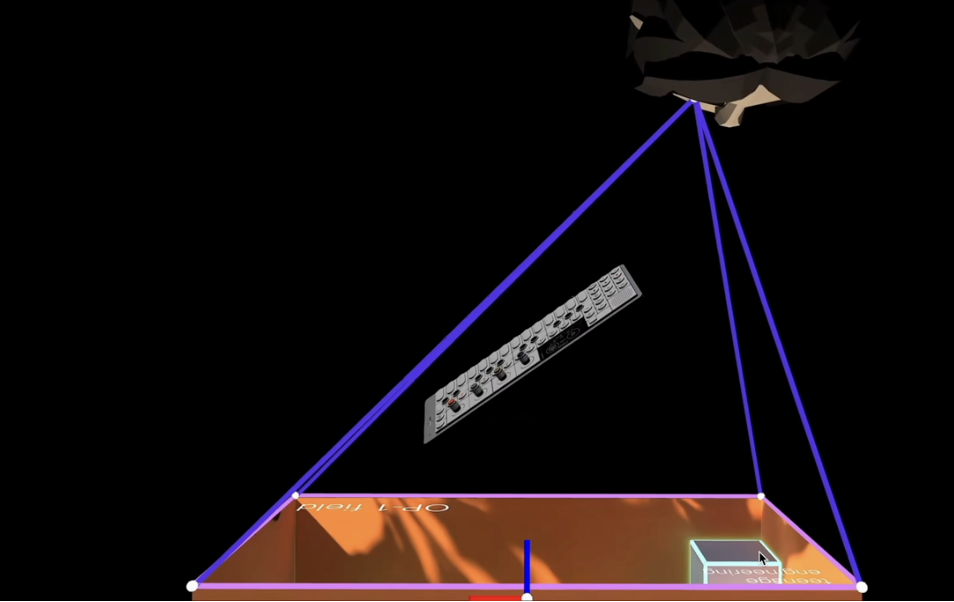
\includegraphics[width=1\textwidth]{figures/example1.png}
            \caption{Principle}\label{F:test-b-sub-a}
        \end{subfigure}
        \begin{subfigure}[t]{.45\linewidth}
            \centering
            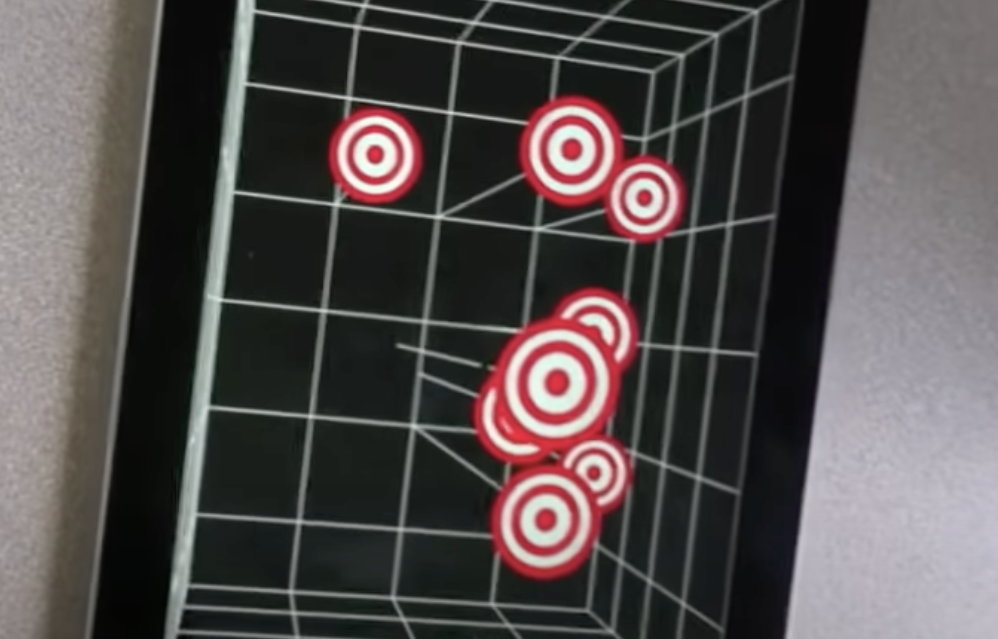
\includegraphics[width=1\textwidth]{figures/image.png}
            \caption{Effect}\label{F:test-b-sub-b}
        \end{subfigure}
        \caption{}\label{F:test-b}
    \end{figure}

    Two keypoint of system are:
    \begin{itemize}
        \item \textbf{Real-time}: System should be able to provide a real-time experience for users.
        \item \textbf{Stable}: Image displayed should be stable, which means image will refresh correctly based on user head's position.
    \end{itemize}

\section{Algorithm Comparison}

\subsection{Face Landmark Detection}
As section 2.1 and section 3 mentioned, face landmark detection should be real-time and precise enough.

\subsection{Pose Estimation}
\lipsum[0]

\subsection{Head Tracking}
\lipsum[0]

% \subsection{Face  Landmark Detection}

% \subsection{Monocular Distance Measuring}

% \subsection{Filter}

% \subsection{Rendering}
